
%%%%%%%%%%%%%%%%%%%%%%%%%%%%%%%%%%%%%%%%%
% задача оптимального выбора группы объектов и алгоритм для её решения
%%%%%%%%%%%%%%%%%%%%%%%%%%%%%%%%%%%%%%%%%
\subsection{Проблема выбора объектов}

Деятельность любых экономических субъектов, будь то организации, предприятия, госкорпорации, научные институты, домашние хозяйства или частные лица, направлена на получение выгоды за счёт затраты определённых ресурсов. Как правило, выгоду нужно максимизировать, а ресурсы ограничены сверху. 

Значительная часть ресурсов выделяется на инвестиции, т.\,е. покупку, развитие или создание неких объектов: промышленных и научных приборов, ценных бумаг, объектов недвижимости и т.\,д. А значит, встаёт проблема оптимального выбора группы объектов, которые будут приобретены, из некого множества $O$ исследуемых объектов, доступных для выбора. Слово <<группа>> в названии настоящей работы и применительно к объектам инвестиций не подразумевает  математическое понятие группы; с точки зрения математики имеется в виду подмножество $d \subset O$. 

За проведение выбора отвечает лицо, принимающее решение. Выбор может стать тривиальным, если объекты достаточно простые с точки зрения оценки выгоды от их приобретения. Но на практике выгода (или потери) от приобретения того или иного объекта часто бывает не очевидна. Приходится работать в условиях неопределённости, когда объективной информации не достаточно для поиска оптимального решения, и важным подспорьем становится субъективные суждения людей, разбирающихся в специфике исследуемых объектов. Лицу, принимающему решение, может потребоваться поддержка экспертов. 

В настоящей работе рассмотрен следующий сценарий: экспертов просят математически выразить субъективное суждение по поводу каждого объекта $i \in O$. Так называемая субъективность суждения эксперта не подразумевает запрета опираться в том числе и на объективную информацию: факты об исследуемых объектах, факты о предметной области в целом, факты о прошлом опыте удачного и неудачного выбора объектов. Но в математической модели экспертной оценки мы не учитываем такую информацию и считаем, что эксперт извлекает оценку непосредственно из своего сознания. 
% к этому абзацу нужны ссылки на другие примеры экспертных заданий в литературе

Каждому объекту $i \in O$, в том (гипотетическом) случае, если бы мы всё о нём знали, можно сопоставить некоторую числовую характеристику целесообразности выбора этого объекта, которую для краткости будем называть <<качеством>> объекта. Разумеется, на самом деле <<качество>> объектов заранее неизвестно, и экспертам предлагается выставить его оценку. Они способны сделать это в силу своего опыта и глубоких знаний предметной области.

Для моделирования заранее неизвестных величин существуют разные математические теории, но в любом случае принято разделять неизвестный математический объект и его истинное числовое значение. Истинное значение <<качества>> $i$-го объекта --- это число $x_i \in X$, где $X$ --- некоторое наперёд заданное числовое множество. Неизвестность $x_i$ в настоящей работе моделируется нечётким элементом $\tilde x_i$ в рамках теории возможностей Ю.~П.~Пытьева. Для $\tilde x_i$ в процессе экспертизы восстанавливается распределение возможности $p_{\tilde x_i}(\cdot): X \rightarrow \zo$. Именно оно и выступает в роли экспертной оценки <<качества>> объекта $i$.  

%Хотя можно представить себе ситуацию, когда это не так... 
Часто <<качество>> объекта, выраженное всего одним, хоть и нечётким, элементом --- недостаточно конкретное и осмысленное понятие. Поэтому заказчик экспертного опроса в качестве предварительного этапа работы с экспертами или до обращения к ним выявляет некоторые {\sl параметры} оцениваемых объектов, часто называемые также <<критериями>> оценки. Будем исходить из того, что каждый объект $i \in O$ можно оценить по одним и тем же $m$ параметрам: $x_{i1} \in X_1, \mydots, x_{im} \in X_m$.  Поскольку заказчику экспертизы важно не только то, какие параметры объектов оценивают эксперты, но и то, как эти параметры формируют итоговую оценку $x_i$, он разрабатывает формулу: $x_i = f(x_{i1}, \mydots, x_{im})$. Например, если все параметры имеют одинаковую важность, можно положить $x_i = \frac{1}{m}\sum_{j=1}^m{x_{ij}}$. На функцию $f(\cdot): X_1 \times \mydots \times X_m \rightarrow X$ могут накладываться ограничения в зависимости от алгоритма, используемого для обработки оценок. 

%Экспертные оценки бывают разные по информативности и существуют разные математические теории для их моделирования  и анализа... этой хрени достаточно во вводных разделах 

Итак, в настоящей работе используется следующая методика экспертного опроса:
\begin{center} \fbox{ 
\begin{minipage}{0.9 \textwidth}
 Экспертам предлагается выставить оценку в виде отображения $X \rightarrow \zo$ для каждого параметра каждого объекта из множества $O$. Эти оценки моделируются и анализируются с помощью теории возможностей Ю.~П.~Пытьева, причём никакая информация, кроме самих экспертных оценок, не учитывается в модели. Делается вывод о том, приобретение какие объектов является наиболее выгодным для заказчика экспертного опроса и можно ли сделать такой выбор.
\end{minipage}
} \end{center}

Подробнее о принятии решений, поддержке принятия решений и причинах возникновения неопределённости написано в разделе \ref{sec:basic_intro}. Примеры практических ситуаций, где требуется сделать выбор в условиях неопределённости, приведены в разделе {}. Подробнее об используемых математических методах теории возможностей Ю.~П.~Пытьева и о других моделях экспертных оценок можно прочитать в разделах {}.

Теперь поставим математическую задачу, выражающую суть изложенной проблемы, и опишем компьютерный алгоритм для нахождения её решения. Будем пока считать, что есть только один эксперт, или же есть экспертный коллектив, но он действует единодушно. Если каждый эксперт может действовать независимо и выдаёт свой собственный набор оценок, то перед использованием нижеизложенного алгоритма следует по каждому параметру каждого объекта рассчитать оценку, выражающую коллективное мнение экспертов. Как это можно сделать, описано в разделе {}.

\subsection{Математическая постановка задачи выбора} % Да, слово "объектов" можно здесь не писать

Пусть имеется $n$ объектов, причём множество $O = \{1, \mydots, n\}$ есть множество их индексов, и для оценки <<качества>> объектов приглашён один эксперт. Ему предложено оценить каждый объект по $m$ параметрам, истинные значения которых неизвестны. Лицу, принимающему решение, требуется  выбрать $k$ из $n$ объектов в $O$, $1 \leq k < n$.

Пусть моделью параметров служат нечёткие элементы $\tilde x_{ij}$. Не ограничивая общности, будем считать, что все они принимают значения на одном и том же числовом множестве $X$, т.\,е. значения параметров имеют вид $x_{ij} \in X$ для параметра с номером $j \in \{1, \mydots, m\}$ объекта с номером $i \in \{1, \mydots, n\}$. Экспертом заданы функции распределения $\p_{ij}(\cdot): X \rightarrow \zo$ нечётких элементов $\tilde x_{ij}$. 

%T состоит из векторов t, а Омега из событий вида {тета=t}, но у них одинаковая размерность.
Введём нечёткий вектор $\theta = \tetavector$, принимающий значения на множестве $T = X^{n \times m}$, которое состоит из всевозможных векторов $t = \tvector$. Будем считать, что его компоненты попарно независимы, что предполагает попарную независимость как параметров каждого объекта, так и самих объектов. Тогда $\theta$ имеет распределение: 
\begin{equation} 
	\label{e:p_theta_def}
	\p_{\theta}\big(\tvector\big) = \inf_{i, j}\,\p_{ij}(x_{ij}),
\end{equation}
и порождает пространство с возможностью $\OAP$, где $\Om$ состоит из элементарных событий вида $\{\theta = t\}$ для всех $t \in T$, причём $\dim \Om = \dim T$. Мера возможности любого события $A \subset \Om$ выражается через $\p_{\theta}(\cdot)$: 
\begin{equation} 
	\label{e:P_theta_def}
	\P(A) = \underset{t\footnotemark \in A} \sup\;\p_{\theta}(t). 
\end{equation}
\footnotetext{Здесь и в дальнейшем изложении будем для краткости использовать обозначение $t$ и для числовых векторов, и для событий вида $\{\theta = t\}$.}
 
Пространство $\OAP$ можно интерпретировать как модель нечёткого эксперимента $\Exp$. Эксперимент  заключается в измерении истинных значений параметров всей совокупности объектов. В реальности он никогда не проводится, т.\,к. его проведение означало бы приобретение сразу всех объектов. Эксперт восстанавливает возможностную модель эксперимента $\Exp$. Наблюдаемые величины и априорная информация отсутствуют в нашей модели эксперимента.

<<Качество>> $i$-го объекта, или итоговую целесообразность его приобретения, будем представлять в той же шкале значений $X$, что и отдельные параметры объекта. Рассмотрим <<качество>> $i$-го объекта $\tilde x_i(\cdot): T \rightarrow X$ при фиксированном $i \in \setN$ как функцию нечётких векторов $\theta = \tetavector$. Перейдём к значениям нечётких элементов: $x_i(t)$ выражается через некоторые из координат вектора $t = \tvector$, а именно $x_{ij}$, $j = \dotM$, с помощью заданной заказчиком экспертизы монотонной по каждому аргументу (требование к заказчику экспертизы) функции $f(\cdot): X^m \rightarrow X$:
\begin{equation}
  \label{e:function_f}
   x_i~\big((x_{11}, \mydots, x_{nm})\big) = f(x_{i1}, \mydots, x_{im}),\,i = \dotN.
\end{equation}
% Поскольку $x_i$ зависит от координат вектора $t$ исключительно через $f$ (и не вообще зависит от $x_{i'j}, i' \neq i$), то $x_i$ также монотонна по всем координатам своего аргумента.    

Требуется выбрать $k$ из $n$ объектов в $O$, $1 \leq k < n$, т.\,е. подмножество $d \subset O$ размера $\abs{d} = k$. Множество всех таких подмножеств обозначим буквой $D$. Допустим, мы знали бы реализацию $\theta = t$ и истинные значения <<качества>> объектов: $x_1 = x_1(t), \mydots, x_n = x_n(t)$. Тогда правильным выбором было бы подмножество строго наиболее <<качественных>> объектов:
\begin{equation}
    \label{e:delta_def}
    \delta_{t} \define= \{i_1, \mydots, i_k\}: \forall\, i \in \delta,\; \forall\, i' \in O \setminus \delta: x_i > x_{i'}. 
\end{equation}
Подмножество $\delta_{t}$ будем называть верным решением задачи выбора {} при $\theta = t$, а объекты $i_1, \mydots, i_k$~--- лидерами. % тире в русском языке не переносится на другую строку
%Если какой-то объект $i \in \delta_t$, будем говорить, что $i$-й объект попал (или вошёл) в $k$ лидеров.

Верное решение существует не всегда. Действительно, если расположить $x_1, \mydots, x_n$ в порядке невозрастания, из определения (\ref{e:delta_def}) следует:
\begin{equation}
   \label{e:right_order_strict}
    \delta_t = \{i_1, \mydots, i_k\}: x_{i_1} \geq \mydots \geq x_{i_k} > x_{i_{k+1}} \geq \mydots \geq x_{i_n},   
\end{equation}
то есть между $x_{i_k}$ и $x_{i_{k+1}}$ должен стоять знак строгого неравенства. Но при некоторых $t$, $k$ возможна такая ситуация:
\begin{equation}
    \label{e:right_order_fail}
    x_{i_1} \geq \mydots \geq x_{i_k} = x_{i_{k+1}} \geq \mydots \geq x_{i_n},    
\end{equation}
и тогда не существует подмножества $\delta_t \subset O$ размера $\abs{\delta} = k$, которое  удовлетворяло бы (\ref{e:delta_def}). Это значит, что при таких $t$ и $k$ нельзя выбрать ровно $k$ лидеров. 

Пусть $\Eps(d)$ --- событие, при котором $d \in D$ является ошибочным решением. Выражение для $\Eps(d)$ получается с помощью отрицания (\ref{e:delta_def}):
\begin{equation}
  \label{e:Eps_d_def}
  \Eps(d) \define= \{t: \exists\, i \in d,\; \exists\, i' \in O \setminus d: x_i(t) \leq x_{i'}(t)\}.
\end{equation}
Словами это означает, что решение ошибочно в том случае, когда для одного из выбранных объектов существует не менее <<качественная>> замена из числа не выбранных объектов.

Можно дать и другое определение. Пусть $\Eps(d)$ --- событие, при котором $d \in D$ не является верным решением:
\begin{equation}
  \label{e:Eps_d_def2}
  \Eps(d) \define= \big\{\{t: \exists\; \delta(t) \neq d\} \cup \{t: \nexists\; \delta(t)\}\big\}. 
\end{equation}
Определения (\ref{e:Eps_d_def}) и (\ref{e:Eps_d_def2}) эквивалентны и взаимозаменяемы.

%Если верного решения не существует, событие $\Eps(d)$ реализуется $\forall\; d \in D$.

Поскольку в реальности $\Exp$ не проводится и реализации нечётких элементов неизвестны, мы не можем найти верное решение, но можем найти оптимальное решение. Согласно (\ref{e:P_theta_def}), через заданные экспертом функции $\p_{ij}(\cdot): X \rightarrow \zo$, $i = \dotN$, $j = \dotM$ можно выразить возможность любого события.  Итак, поставим задачу (оптимального) выбора {} как задачу минимизации возможности события $\Eps(d)$:
\begin{equation}
  \label{e:zadacha}
  \P(\Eps(d)) \sim \underset{d \in D} \min.
\end{equation}

\subsection{Решение математической задачи выбора}

Зафиксируем объект с номером $l \in O$ и конкретную реализацию  $t$ нечёткого вектора $\theta$. Пусть $\pi_l(t) \in \setN$ --- это количество таких объектов, <<качество>> которых не меньше $x_l(t)$, считая сам $l$-й объект:
\begin{equation}
  \label{e:Eps_l_def}
  \pi_l(t) \define=  \abs{L'}, L' = \{l': x_l'(t) \geq x_{l}(t)\}  \subset O.
\end{equation}
 Число $\pi_l(t)$ зависит только от упорядоченности значений <<качества>> объектов из $O$, а не от конкретных значений <<качества>>. Эта упорядоченность, в свою очередь, зависит от $t$. \begin{comment} Вот несколько простых примеров вычисления значения функции $\pi_l(\cdot): T \rightarrow \setN$:
\begin{itemize}
  \item $x_l(t) > x_i(t) \;\forall\, i \neq l \Rightarrow \pi_l(t) = 1$;
  \item $x_{l'}(t) = x_l(t) > x_i(t) \;\forall\, i \neq l,\; i \neq l' \Rightarrow \pi_l(t) = 2$;
  \item $x_{l'}(t) > x_l(t) > x_i(t) \;\forall\, i \neq l,\; i \neq l' \Rightarrow \pi_l(t) = 2$;
  \item $x_l(t) < x_i(t) \;\forall\, i \neq l \Rightarrow \pi_l(t) = n$;
  \item $x_l(t) = x_i(t) \;\forall\, i \Rightarrow \pi_l(t) = n$.
\end{itemize}

\end{comment}

%\item Наконец, нам понадобится такое утверждение:
%  \begin{equation}
%    \label{e:if_leader}
%	 x_{i_1} \geq \mydots \geq x_{l} \geq \mydots \geq x_{i_k} > x_{i_{k+1}} \geq \mydots \geq x_{i_n} 
%    (\ref{right_order_strict}) \Rightarrow \pi_l(t) \leq k.
%  \end{equation}
%Последнее означает, что если при $\theta = t$ существует верное решение задачи выбора объектов (\ref{right_order_strict}), и объект с номером $l$ является одним из лидеров, то $\pi_l(t) \leq k$.

Введём следующий набор событий:
\begin{equation}
  \label{e:Eps_l_def}
  \Eps_l \define= \{t: \pi_l(t) > k\} = \{t: \exists\, L' \subset O, \abs{L'} > k: \forall\, l' \in L'\;x_l'(t) \geq x_{l}(t)\}.
\end{equation}

Докажем, что при произвольном $t$, заранее фиксированное решение $d \in D$ ошибочно тогда и только тогда, когда для одного из выбранных объектов $l \in d$ реализуется событие $\Eps_l$.
\begin{enumerate}
  \item Если $\exists\, \delta_t$, удовлетворяющее~\eqref{e:right_order_strict}, реализация события $\Eps_l$ означает $l \notin \delta_t$.
  Действительно, по определению $\Eps_l$ верно $\pi_l(t) > k$, а если бы объект с номером $l$ был одним из $k$ лидеров, выполнялось бы $\pi_l(t) \leq k$, поскольку $\abs{\delta_t} = k$. Отсюда следует, что при $l \in d$ реализуется $\Eps(d)$~(\ref{e:Eps_d_def2}).
  \item Если $\nexists\, \delta_t$, т.\,е. выполняется~(\ref{e:right_order_fail}), то $\pi_l(t) > k$, вообще говоря, не означает, что <<качество>> $l$-й объекта меньше <<качества>> остальных объектов. Но если верного решения не существует, событие $\Eps(d')$ по определению~\eqref{e:Eps_d_def2} реализуется $\forall\; d' \in D$, в том числе при $d' = d$. 
  \item Если же решение $d$ ошибочно (не важно, существует ли $\delta_t$), то в силу~(\ref{e:Eps_d_def}) $\exists\, i \in d,\, i' \notin d: x_i(t) \leq x_{i'}(t)$. %Для этого $l$ и реализуется $\Eps_l$. % А вот и нет)))
  Пусть $l = \arg\min \{x_{l'}(t)\mid\,l' \in d\}$, для него уже $\pi_l(t) \geq k$ в силу $\abs{d} = k$. Но $x_l(t) \leq x_i(t) \leq x_{i'}(t)$, откуда $\pi_l(t) \geq k+1$ и реализуется событие $\Eps_l$.     
\end{enumerate}

Поскольку событие $\Eps(d)$ реализуется тогда и только тогда, когда реализуется одно из событий $\Eps_l, l \in d$, оно может быть представлено в виде
\begin{equation*}
  \Eps(d) = \bigcup_{l \in d} \Eps_l.
\end{equation*}

Наконец, перейдём к возможностям рассматриваемых событий, а именно запишем связь между минимизируемой $\P(\Eps(d))$ и возможностями событий $\Eps_l$. Несмотря на то, что, вообще говоря, $\Eps_l \cap \Eps_l' \neq \varnothing,\; l \neq l'$, правило суммирования возможностей позволяет записать:
\begin{equation}
  \label{e:razbienie}
  \P(\Eps(d)) = \sup_{l \in d} \P(\Eps_l).
\end{equation}

Предположим, мы рассчитали  $\P(\Eps_l)$ для каждого объекта $l \in O$ и отсортировали объекты по неубыванию этих величин:
\begin{equation}
  \label{e:left_order}
  \P(\Eps_{l_1}) \leq ... \leq \P(\Eps_{l_k}) \leq \P(\Eps_{l_{k+1}}) \leq ... \leq \P(\Eps_{l_n}). 
\end{equation}
Тогда $d_* = \{l_1, ...,  l_k\}$ будет решением задачи (\ref{e:zadacha}). Действительно, положив в (\ref{e:razbienie}) $d = d_*$, получим $\P(\Eps(d)) = \P(\Eps_{l_k}) = P_*$, а заменив какой-нибудь элемент  решения на $l_r$, $r > k$, получим $\P(\Eps(d)) = \P(\Eps_{l_r}) \geq P_*$. 

\subsubsection*{Замечание}
\begin{notice}
%Может возникнуть неоднозначность выбора $d_*$, связанная с наличием знаков равенства в цепочке (\ref{e:left_order}). 
Пусть в цепочке (\ref{e:left_order}) $P_* = \P(\Eps_{l_k}) = ... = \P(\Eps_{l_q}) < \P(\Eps_{l_{q+1}})$, $q \geq k$. По построению минимум (\ref{e:zadacha}) достигается на любом решении $d' \subset \Delta \define= \{l_1, ..., l_q\}$, $\abs{d'} = k$, и такое $d'$ сводится к $d_*$ простой заменой индексов. Если $q > k$, следует считать, что решение задачи оптимального выбора объектов не единственное, и сообщить об этом заказчику экспертного опроса. Лицо, принимающее решение, может или отказаться от выбора вовсе, например, потребовав дополнительную экспертизу, или выбрать любые $k$ объектов из $\Delta$, или даже отказаться от исходного требования задачи и вместо $k$ выбрать $r$ объектов из $\Delta$, где $k \leq r \leq q$.
\end{notice}
%\subsection{Алгоритм нахождения возможности не попасть в число лидеров}

 Итак, задачу (\ref{e:zadacha}) мы свели к задаче нахождения $\P(\Eps_l)$, $l = \dotN$. В соответствии с (\ref{e:p_theta_def}), (\ref{e:P_theta_def}):
\begin{equation}
  \label{e:pl_main}
  \P(\Eps_l) = \sup_{(x_{11}, ..., x_{nm})\,\in\,\Eps_l} \, \inf_{i, j}\,\p_{ij}(x_{ij}). 
  % заданы какие-то конкретные параметров x_{ij}, и уже потом по ним берётся супремум, поэтому p_{ij}(x_{ij}) 
  % эксперт же задаёт p_{ij}(x) при всех значениях х, т.е. функции p_{ij}()
\end{equation}

Узким местом формулы~(\ref{e:pl_main}) при вычислении <<в лоб>> является перебор всех векторов $t \in T$ для проверки на предмет включения в $\Eps_l$. Если $X$ имеет мощность континуума, то и $T$ имеет мощность континуума. Даже в случае конечного множества $X$ перебор всех векторов невозможен, поскольку $\abs{T} = \abs{X}^{nm}$. Но оказывается, для приближённого нахождения $\P(\Eps_l)$\footnote{В представляющем интерес <<дискретном>> частном случае будет найдено не приближённое, а точное значение $\P(\Eps_l)$ --- это объясняется ниже.} с точностью $\varepsilon = 2^{-N}$ полный перебор делать не нужно: достаточно перебрать всего $N-1$ векторов, причём множество $X$ даже {\sl не обязано} быть конечным. Дело в том, что можно относительно просто проверить отношение $\P(\Eps_l) > p$ для любого заданного числа $p \in \zo$ в силу транзитивности операций сравнения действительных чисел, лежащих в основе <<работы>>  $\sup$ и $\inf$, и монотонности функции $f$ в формуле~(\ref{e:function_f}) по всем аргументам. 

\subsection{Быстрый алгоритм поиска возможностей}

В общем случае любая возможность лежит на отрезке $\zo$. Будем искать $\P(\Eps_l)$ отдельно для каждого конкретного $l \in O$ методом дихотомии. В качестве начального приближения $p^{(0)}$ возьмём середину отрезка $[p^{min(0)}, p^{max(0)}] = \zo$. На $i$-ой итерации алгоритма, где $i = 0, \ldots, N$, специальным образом проверяем утверждение $\P(\Eps_l) > p^{(i)}$, и в зависимости от результата проверки продолжаем поиск на одной из половин $[p^{min(i)}, p^{(i)}]$ или $[p^{(i)}, p^{max(i)}]$. Таким образом, каждый следующий отрезок поиска в два раза короче предыдущего.  На $N$-ой итерации $\abs{p^{max(N)} - p^{min(N)}} < 2^{-N}$, и можно положить $\P(\Eps_l) \approx p^{(N)}$. Если в качестве независимого параметра задано не $N$, а максимальная погрешность  $\varepsilon$, следует взять $N = N_{\varepsilon} = [\log_2{\varepsilon}]+1$,  где квадратные скобки означают взятие целой части от выражения. 

Трудности при интерпретации приближённых значений возможности могли бы возникнуть в следующих случаях:
\begin{enumerate}
  \item когда истинное значение $\P(\Eps_l)$ равно $0$ или $1$, поскольку эти числа имеют особый смысл в теории возможностей,
  \item когда для каких-либо $l_1 \neq l_2: \P(\Eps_{l_1}) = \P(\Eps_{l_2})$.
\end{enumerate}

Но, во-первых, при анализе совокупности результатов $p^{(N)}$ и $[p^{max(N)} - p^{min(N)}]$ для разных $l$ такие случаи часто хорошо видны. Во-вторых, во многих практически важных случаях область значений возможности дискретна, и можно получить не приближенное, а точное значение $\P(\Eps_l)$. 

Пусть в качестве $X$ выбрано конечное множество, например, $X = \{0, 1, \ldots, x_{max}\}$. Тогда множество всех элементарных событий $\Omega$ конечно, хотя имеет большой размер: $\abs{\Omega}= \abs{T} = \abs{X}^{nm}$. Множество значений возможностей элементарных событий $Y = \{\p(\omega) \define= \P(\{\omega\})\mid\omega\in\Omega\}$ тоже конечно, имеет тот же размер и состоит из отдельных точек отрезка $\zo$. 
\begin{comment} 
Возьмём 
\begin{equation*}
  \label{e:N_for_second_case}
  N_Y = [ \log_{2}{\abs{X}^{nm}} ] + 1 =
      nm[ \log_{2}{x_{max}} ] + 1,
\end{equation*}
где квадратные скобки означают взятие целой части от выражения.
\end{comment}
При достаточно большом $N$, на $N$-ой итерации метода дихотомии найдётся единственное число $\p(\omega)\in[p^{min(N)}, p^{max(N)}]$. Поскольку операции $\sup$ и $\inf$ над значениями возможности не выводят за пределы исходного множества чисел $\{\p(\omega) \mid\omega\in\Omega\}$, тем самым автоматически будет найдено значение $\P(\Eps_l) \in [p^{min(N)}, p^{max(N)}]$.  

Можно показать, что в наихудшем случае для произвольного $Y$ количество итераций дихотомии равно $\abs{Y}$. 
Действительно, пусть на самом деле $\P(\Eps_l) = 0$, что вынуждает алгоритм каждую итерацию продолжать поиск на левой половине $[p^{min}, p^{max}]$, а множество $Y$ устроено так: на отрезке $[0.5;  1]$ лежит только одна точка из $Y$, на отрезке $[0.25;  0.5]$ --- ещё только одна точка, на отрезке $[0.125;  0.25]$ --- третья точка и т.\,д. Лишь на итерации $N = \abs{Y}$ в нужной половине $[p^{min}, p^{max}]$ останется только точка <<$0$>>. 

Но принцип относительности из теории возможностей позволяет изящно избежать эту ловушку. Содержательно интерпретируется только упорядоченность чисел $\p(\omega), \omega\in\Omega$. Поэтому возьмём множество $Y' = \{\p'(\omega) \define= \gamma(\p(\omega))\mid\omega\in\Omega\}$, где $\gamma(\cdot): \zo \to \zo$ выбирается согласно определению () таким образом, что возможности элементарных событий $p'$ уже распределены равномерно по отрезку~$\zo$ (с точностью до совпадающих точек --- равновозможных элементарных событий). Между $Y$ и $Y'$ установлена биекция. На вход алгоритма дихотомии подаётся $Y'$, поиск на котором отвечает наилучшему случаю дихотомии с количеством итераций, равном:
\begin{equation*}
  \label{e:}
  [ \log_{2}{\abs{X}^{nm}} ] + 1 = nm[ \log_{2}{x_{max}} ] + 1,
\end{equation*}
 где квадратные скобки означают взятие целой части от выражения.
 
%$\Theta(\log_{2}{\abs{X}^{nm}}) =  \log_{2}{x_{max}}\Theta(nm)$\footnote{Символы $\Theta(g(nm))$ обозначают асимптотически точную оценку. График зависимости количества итераций $N$ от размера $nm$ массива входных данных при $nm \to\infty$ лежит не ниже кривой $N = С_1g(nm)$ и не выше кривой $N = С_2g(nm)$, $C_1 < C_2$.}.  
%\todo{Эту проблему легко решить при конечном $Y$. Для этого надо просто распределить значения возможностей равномерно по отрезку $[0,1]$, то есть использовать вместо $Y$ более <<удобное>> множ. $Y'$. Между $Y$ и $Y'$ установлена биекция. Надо об этом написать.}\xspace  \todo{А вот это убрать, т.\;к. это очень нестрогие рассуждения.}Конечно, на практике такое встречается редко, и в среднем при равномерном распределении точек из $Y$ на отрезке $\zo$ \todo{Разъяснить, что $\to\infty$}\colorbox{green}{асимптотическая} сложность алгоритма  равна $\log_{2}{\abs{X}^{nm}} =  nm \log_{2}{x_{max}}$.

Можно ещё больше упростить ситуацию даже в случае произвольного $X$. Достаточно <<вручную>> вместо непрерывного множества значений возможности $\zo$ взять конечный набор, например, $Y = \{0.0, 0.1, \ldots, 1.0\}$. Операции $\sup$ и $\inf$ не выводят за пределы $Y$, поэтому $\P(\Eps_l) \in Y$, если исходный материал --- экспертные оценки $\p_{ij}(\cdot): X \rightarrow Y$ (что в определённом смысле удобно и для экспертов). В нашем примере $Y = \{0.0, 0.1, \ldots, 1.0\}$, поэтому уже при $N = 5 \Rightarrow 2^{-N} < 0.05$ можно $p^{(N)}$ однозначно отнести к $\P(\Eps_l) \in Y$.

%$[p^{min(N_{\varepsilon})}, p^{max(N_{\varepsilon})}]$
Итого, будем использовать следующую модификацию метода дихотомии (см. рисунок \ref{ris:algo_scheme}). Если пользователем задан параметр $\varepsilon > 0$, ищется приближённое значение $\P(\Eps_l)$, попадающее в отрезок $[p^{min}, p^{max}]$ шириной не более $\varepsilon$. Если задано отрицательное значение $\varepsilon$, пользователь должен указать конечное множество $Y$, на котором лежат значения всех возможностных мер, и алгоритм фиксирует момент, когда в отрезок $[p^{min}, p^{max}]$ попадает только один элемент $p' \in Y$. %Здесь номер итерации $i$ пробегает значения $1, \ldots, N_Y$, а если \todo{Это как?}\colorbox{green}{после достижения $N_Y$ ответ не найден, считается, что допущена ошибка в исходных данных}. 

\begin{figure}[h!]
\center{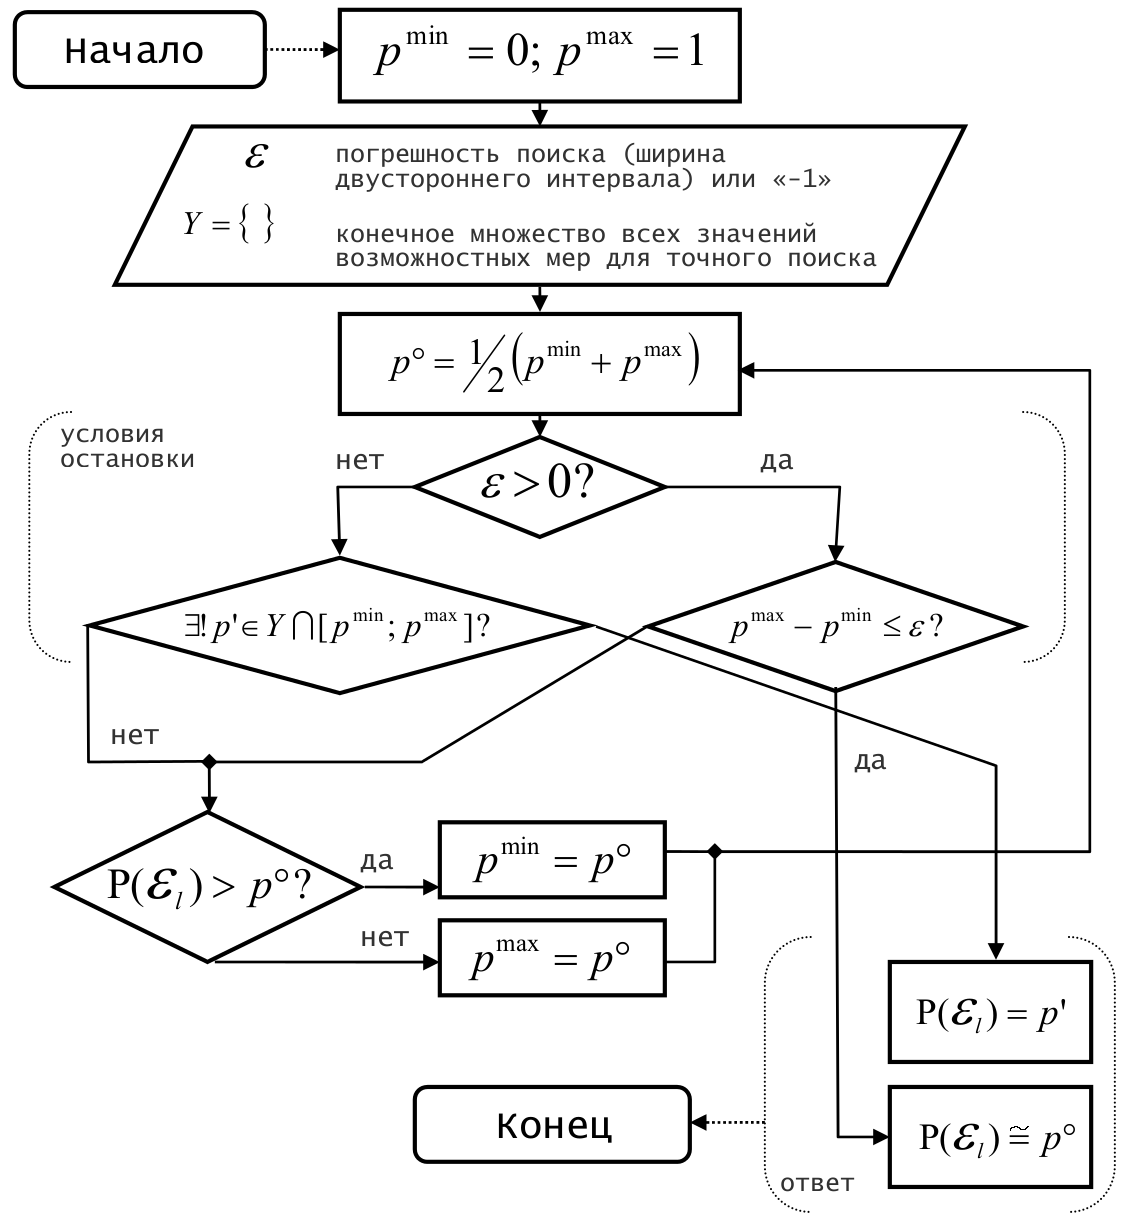
\includegraphics[width=0.75\linewidth]{./pic/block-scheme}}
\caption{\small Принципиальная блок-схема применяемого алгоритма дихотомии. Некоторые незначительне действия,, например, расчёт максимального количество итераций и проверка на его достижение, здесь опущены. В зависимости от того, задано ли положительное значение $\varepsilon$ и множество всех значений возможностных мер $Y$, алгоритм может искать приближённое или точное значение $\P(\Eps_l)$. <<Сердцем>> алгоритма является проверка утверждения $\P(\Eps_l) > p$.}
\label{ris:algo_scheme}
\end{figure}

%Пусть на $N$-ой итерации дихотомии $p^{(N)} = p \in \zo$.
Пусть $p \in \zo$. <<Сердцем>> алгоритма является проверка утверждения $\P(\Eps_l) > p$. Чтобы узнать, верно ли это утверждение, выполним следующие действия: 
\begin{enumerate}
  \item 
  Для каждого $i \in \{1, ..., n\}$, $j \in \{1, ..., m\}$ найдём подмножество $X_{ij} \define= \{x \in X: p_{ij}(x) > p\} \subset X$. 
  \item 
  Определим $t^\text{edge} = (x_{11}^\text{edge}, \mydots, x_{nm}^\text{edge})$ следующим образом:
  \begin{equation*}
    x_{ij}^\text{edge} =
    \begin{cases}
      \min X_{ij}, &\text{если $i = l$.}\\
      \max X_{ij}, &\text{если $i \neq l$.} 
    \end{cases}
  \end{equation*}
  Элементарное событие, которому соотвествует вектор $t^\text{edge}$, заключается в том, что параметры $j$ объекта $l$ приняли минимальные значения среди $X_{lj}$, а каждый параметр $j$ всех остальных объектов $i \neq l$, наоборот, принял максимальное значение в <<своём>> множестве $X_{ij}$. 
  \item	%не совпадающих с $l$-м, %%ни фига, сверил с кодом
  Вычислим значение $\pi_l(t^\text{edge})$: 
 	\begin{itemize}
		\item если $\pi_l(t^\text{edge}) > k$, то $\P(\Eps_l) > p$.
		\item в противном случае, $\P(\Eps_l) \leq p$.
	\end{itemize} 
\end{enumerate}  

Проясним смысл этих действий. Поскольку в теории возможностей верно
\begin{equation*}
 % \label{e:transitive}
  \P(A) > a \Leftrightarrow \exists\, \omega \in A: \p(\omega) > a,
\end{equation*}
то в силу (\ref{e:pl_main}) утверждение $\P(\Eps_l) \leq p$ истинно, если и только если у всех векторов $t = \tvector \in \Eps_l$ хотя бы одна координата $x_{ij}$ такова, что $\p_{ij}(x_{ij}) \leq p$. Построим отрицание к сказанному: $\P(\Eps_l) > p$ истинно, если и только если найдётся хотя бы один вектор $t \in \Eps_l$, у которого все координаты $x_{ij} $ будут лежать в соответствующих подмножествах $X_{ij} = \{x \in X: p_{ij}(x) > p\}$, $i = \dotN$, $j = \dotM$.
%\begin{equation}
%  \label{e:P_greater_p}
%  \P(\Eps_l) > p \Leftrightarrow \exists\; t = (x_{11}, \mydots, x_{nm}) \in \Eps_l: \forall\; i = \dotN, j = \dotM  x_{ij} \in X_{ij} = \{x \in X: p_{ij}(x) > p\}.
%\end{equation}

Координаты $x_{ij}^\text{edge}$ вектора $t^\text{edge}$ по построению лежат в соответствующих подмножествах $X_{ij}$. Поэтому если $t^\text{edge} \in \Eps_l$, сразу делается вывод $\P(\Eps_l) > p$. Докажем, что если $t^\text{edge} \notin \Eps_l$, то и никакой другой вектор $t$ с координатами $x_{ij} \in X_{ij}$ не лежит в $\Eps_l$. 

Функция $\pi_l$ монотонно зависит от каждой координаты вектора $t \in T$ в силу монотонности $f$ по каждому аргументу: она невозрастает при возрастании той группы координат, которая обуславливает возрастание $x_l(t)$, и неубывает при возрастании всех остальных координат. По построению $t^\text{edge}$, изменение каких-либо из координат $x_{ij}^\text{edge}$ в пределах $X_{ij}$ не уменьшает $x_l(t^\text{edge})$ и не увеличивает $x_i(t^\text{edge}), i \neq l$. Поэтому вектору $t^\text{edge}$ соответствует максимально большое значение $\pi_l$ в пределах события $A = \{t = (x_{11}, ..., x_{nm}): x_{ij} \in X_{ij}\}$.

Событие $\Eps_l$ по определению состоит из $t: \pi_l(t) > k$, и либо пересекается, либо не пересекается с $A$, см.~рис.~\ref{ris:algo_sets}. Если $\Eps_l \cap A = \varnothing$, то их можно разделить прямой $\{\pi_l(t) = \pi_l(t^\text{edge})\}$, которая обозначена пунктиром на рисунке. Что и требовалось доказать.

\begin{figure}[h!]
\center{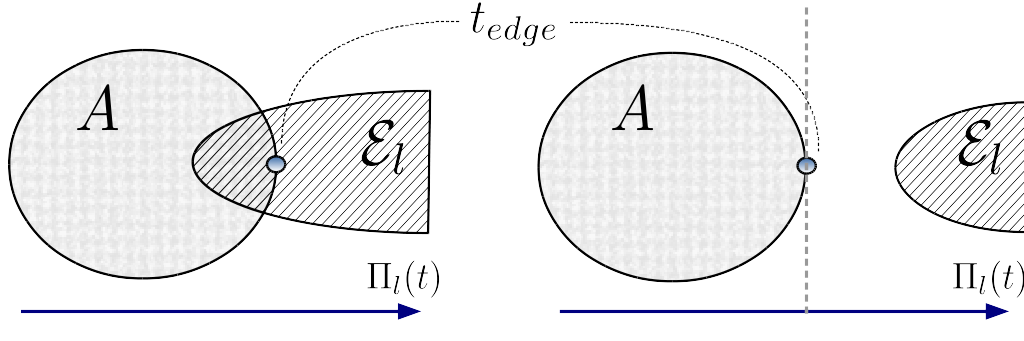
\includegraphics[width=0.85\linewidth]{./pic/algo_sets2}}
\caption{\small Иллюстрация взаимного расположения исследуемых событий и построенного вектора $t_{edge}$ в случае $\P(\Eps_l) > p$ (справа) и в случае $\P(\Eps_l) \leq p$ (слева) для заданного $p \in \zo$.}
\label{ris:algo_sets}
\end{figure}

%\subsection{Анализ корректности решения задачи выбора}
% ==moved up
\begin{comment}
\subsubsection*{Замечание 2}

Пусть $E_0 = \{t: \nexists \delta(t)\}$. Это событие возникает, когда найдётся хотя бы $n-k+1$ объектов, для каждого из которых найдётся $k$ объектов не меньшей <<значимости>>:
\begin{equation*}
 E_0 = (\Eps_1 \cap ... \cap \Eps_{n-k+1}) \bigcup (\Eps_2 \cap ... \cap \Eps_{n-k+2}) \bigcup ... \bigcup (\Eps_{k-1} \cap ... \cap \Eps_{n}).
 % надо было бы объедиение по всем возможным наборам, но всё гораздо проще!
\end{equation*}
Событие $E_0$ --- более узкое, чем $\Eps_l$, где требуется $k$ объектов не меньшей <<значимости>> только для объекта $l$:
\begin{equation*}
 E_0 \subset \Eps_l \Rightarrow \Eps_l = E_0 \cup E_l,\;l \in O,
\end{equation*}
где $E_0$ состоит из векторов $t: \nexists \delta(t)$, которые войдут во все $\Eps_l$, а 
$E_l$ --- оставшаяся часть $\Eps_l$. По правилу сложения возможностей:
\begin{equation*}
 \P(\Eps_l) = \sup\{\P(E_0), \P(E_l)\}.
\end{equation*}
%НЕ СОВСЕМ ВЕРНО: Постоянное первое слагаемое зависит, прежде всего, от выбора $f$ (\ref{e:function_f}). Если оно больше, чем минимум второго слагаемого, для некоторых $l$, возможности таких $\Eps_l$ будут равны, а это может быть плохо для однозначности решения задачи (\ref{e:zadacha}). Поэтому в спорной ситуации, когда в цепочке (\ref{e:left_order}) много равенств, имеет смысл посмотреть на возможность $\P(E_0)$. Если она окажется равна многим $\P(\Eps_l)$, требуется выбрать другую функцию $f$. Если же нет, то спорная ситуация возникла только из-за экспертных $\p_{ij}$.
\end{comment}
